\section{Discussione sui diodi}
\begin{figure}[h]
	\centering
	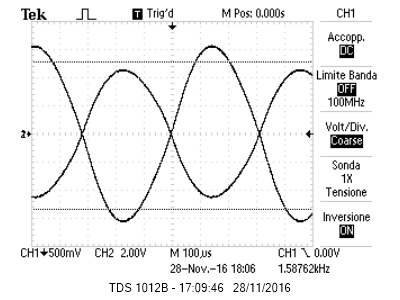
\includegraphics{parte5_con.png}
	\caption{Circuito con entrambi i diodi inseriti.Si osserva l'oscillazione attesa con frequenza discussa nella sezione precedente.}
	\label{f:con_diodi}
\end{figure}	

\begin{figure}[h]
	\centering
	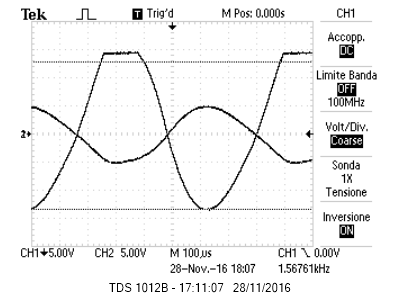
\includegraphics{parte5_senza1.png}
	\caption{Circuito con un solo diodo inserito.Si inizia ad osservare il clipping sull'uscita.}
	\label{f:senza_1diodo}
\end{figure}

\begin{figure}[h]
	\centering
	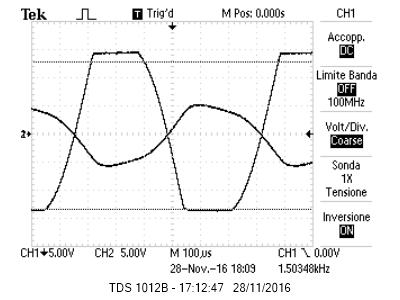
\includegraphics{parte5_senza2.png}
	\caption{Circuito senza diodi. Si nota che l'uscita viene clippata maggiormente rispetto al caso di un solo diodo inserito.}
	\label{f:senza_2diodi}
\end{figure}
Si sono analizzate varie configurazioni del circuito al variare del numero di diodi inseriti. In \fig{con_diodi},\ref{f:senza_1diodo} e \ref{f:senza_2diodi} si osservano le tre configurazioni analizzate.Nel canale uno c'è l'ingresso del generatore mentre sul secondo canale l'uscita $V_{out}$.
Il ruolo dei diodi in tale circuito è quello di evitare che l'uscita vada in saturazione.Infatti per segnali con ampiezza molto maggiore di $V_\gamma \approx 0.6$V la resistenza dei diodi è molto minore di $R_3$ e quindi è equivalente a dire che quest'ultima resistenza è cortocircuitata.Tale effetto diminuisce notevolmente il guadagno. Quindi è normale aspettarsi che rimuovendo i due diodi, non si possa ottenere tale effetto sul guadagno e quindi si osserva il clipping del segnale.
